% ====================================================================
% v7-02b.tex  —  graphite_ica_ch1 v7 (경쟁 구현 02-b)
%   v7-02.tex 에서 보완:
%     (1) 기호 𝒜 이중 의미 해소 — N7 컷점 상수 하나로 통일
%         (N4/N5 eq:stationary 의 전위-의존 구동력은 풀어쓰기로 대체)
%     (2) verifybox §2 분극 peak 위치 결론 부호 교정 (낮은→높은)
%     (3) §8 부호 체크리스트 전건 재확인 + 부호회귀 self-test
%   원본 v7-02.tex 보존, 이 파일은 v7-02.tex 기반 보완본(b).
%   build: xelatex -interaction=nonstopmode (2-pass)
% ====================================================================
\documentclass[11pt,a4paper]{article}
\usepackage[margin=22mm]{geometry}
\usepackage{kotex}
\setmonofont{D2Coding}[Scale=MatchLowercase]
\usepackage{amsmath,amssymb,mathtools,bm}
\usepackage{booktabs,longtable,array}
\usepackage{enumitem}
\usepackage{amsthm}
\usepackage{hyperref}
\usepackage{fancyhdr}
\usepackage{lastpage}
\usepackage{setspace}
\usepackage{tikz}
\usetikzlibrary{positioning,arrows.meta}
\setstretch{1.12}
\setlength{\parskip}{0.45em}
\setlength{\parindent}{0pt}
\setlength{\headheight}{14pt}
\setlength{\emergencystretch}{2em}
\hypersetup{colorlinks=true, linkcolor=blue, urlcolor=blue, citecolor=blue,
  pdftitle={흑연 음극 dQ/dV 이론: v11 코드 기반 수식-구동 --- Chapter 1 (v7-02b)}}
\pagestyle{fancy}\fancyhf{}
\lhead{흑연 음극 $dQ/dV$ 이론 --- Ch.\,1 (v7-02b)}\rhead{\thepage/\pageref{LastPage}}
\renewcommand{\headrulewidth}{0.4pt}

\newtheorem*{keybox}{핵심}
\newtheorem*{verifybox}{검산}
\newtheorem*{boundbox}{유효 범위}

\newcommand{\dd}{\mathrm{d}}
\newcommand{\eff}{\mathrm{eff}}
\newcommand{\eq}{\mathrm{eq}}
\newcommand{\app}{\mathrm{app}}
\newcommand{\cell}{\mathrm{cell}}
\newcommand{\bg}{\mathrm{bg}}
\newcommand{\dis}{\mathrm{dis}}
\newcommand{\chg}{\mathrm{chg}}
\newcommand{\hys}{\mathrm{hys}}
\newcommand{\sstat}{\mathrm{ss}}

\renewcommand{\theequation}{1.\arabic{equation}}
\renewcommand{\thesection}{1.\arabic{section}}

\title{\textbf{\LARGE Chapter 1}\\[0.35em]
  \Large 흑연 음극 $dQ/dV$ 이론:\\[0.2em]
  v11 코드 진행을 절 순서로 삼아 유도하는 수식-구동 교과서판}
\author{}
\date{}

\makeatletter
\renewcommand*\l@section[2]{%
  \ifnum \c@tocdepth >\z@
    \addpenalty\@secpenalty
    \addvspace{1.0em \@plus\p@}%
    \setlength\@tempdima{2.3em}%
    \begingroup
      \parindent \z@ \rightskip \@pnumwidth
      \parfillskip -\@pnumwidth
      \leavevmode \bfseries
      \advance\leftskip\@tempdima
      \hskip -\leftskip
      #1\nobreak\hfil
      \nobreak\hb@xt@\@pnumwidth{\hss #2\kern-\p@\kern\p@}\par
    \endgroup
  \fi}
\renewcommand*\l@subsection{\@dottedtocline{2}{2.3em}{3.2em}}
\makeatother

\begin{document}
\maketitle

% ====================================================================
\section*{서론}
\addcontentsline{toc}{section}{서론}
% ====================================================================
리튬이온전지 흑연 음극의 \textbf{incremental capacity analysis}(ICA)는
충방전 곡선 $Q(V)$의 미분 $\dd Q/\dd V$를 분석한다.
흑연은 staging 상전이(stage $4\!\to\!3\!\to\!2\mathrm{L}\!\to\!2\!\to\!1$)를 거치고,
각 전이에서 두 상이 공존하면 전위가 평탄해지며 좁은 전압 구간에 큰 전하가 몰려
$\dd Q/\dd V$ peak가 형성된다.

본 장의 목표는 \textbf{\texttt{Anode\_Fit\_v11\_final.py}의 코드 계산 진행(N0$\to$N9)을
절 순서로 삼아, 각 단계의 물리식을 그 순서대로 유도}하는 것이다.
독자는 이 문건만으로 v11 곡선을 재현하는 코드를 작성할 수 있어야 한다.
주 전개는 방전(탈리튬화; $\sigma_d{=}{+}1$)이고, 히스테리시스·충전은
방전 위상의 분기로 다룬다.

\tableofcontents
\newpage

% ====================================================================
\section{기호와 규약 (N0: 실험조건 → 모델입력)}
\label{sec:notation}
% ====================================================================
코드 진입 경로 \texttt{curve()} $\to$ \texttt{dqdv()} 의 N0 노드는 실험조건을
모델 입력으로 환산한다. 이 절은 그 환산과 전체 문건에 쓰이는 기호를 정리한다.

\subsection{방향 부호와 전류}
방전 또는 충전 방향을
\begin{equation}
  \sigma_d \;=\; \begin{cases}+1 & \text{방전(탈리튬화)}\\ -1 & \text{충전(리튬화)}\end{cases}
  \label{eq:sigmad}
\end{equation}
로 정의한다 [\texttt{\_direction\_to\_sigma}, L514].
전류 크기 $|I| = C\text{-rate}\times Q_\cell$ [A]이고,
무차원 용량 좌표 $q = \int|I|\,\dd t/Q_\cell \in[0,1]$ 이다.
온도 $T$ [K]는 등온(스칼라) 또는 전위 배열 $T(V)$를 허용한다.

\subsection{기호 사전}
\begin{longtable}{p{0.15\textwidth} p{0.13\textwidth} p{0.64\textwidth}}
\toprule 기호 & 단위 & 의미 \\ \midrule \endhead
\multicolumn{3}{l}{\emph{--- 전역 상수 ---}}\\
$R$ & J/(mol\,K) & 기체상수 $8.314$ \\
$F$ & C/mol & Faraday 상수 $96485$ \\
$k_B$ & J/K & Boltzmann 상수 $1.381\times10^{-23}$ \\
$h$ & J\,s & Planck 상수 $6.626\times10^{-34}$ \\
\multicolumn{3}{l}{\emph{--- 실험조건(N0) ---}}\\
$\sigma_d$ & --- & 방향 부호 (식~\eqref{eq:sigmad}) \\
$|I|$ & A & 전류 크기 \\
$Q_\cell$ & C & 셀 용량 \\
$T$ & K & 온도 \\
$q$ & --- & 무차원 용량 $=\int|I|\,\dd t/Q_\cell$ \\
\multicolumn{3}{l}{\emph{--- 분극(N1) ---}}\\
$V_\app$ & V & 인가(측정) 전위 \\
$V_n$ & V & 내부 전위(열역학 전위; 분극 제거 후) \\
$R_n$ & $\Omega$ & 직렬 저항 [\texttt{Rn}] \\
\multicolumn{3}{l}{\emph{--- 평형(N2) ---}}\\
$j$ & --- & 전이 인덱스 ($j=1,\dots,N_p$; 흑연 $N_p=4$) \\
$U_j(T)$ & V & 전이 $j$의 평형 중심 전위 [\texttt{func\_U\_j}] \\
$\Delta H_{\mathrm{rxn},j}$ & J/mol & 삽입 반응 엔탈피 \\
$\Delta S_{\mathrm{rxn},j}$ & J/(mol\,K) & 삽입 반응 엔트로피 \\
\multicolumn{3}{l}{\emph{--- 폭·점유(N4, N5) ---}}\\
$n_j$ & --- & 폭 다중도 [\texttt{\_n\_factor}] \\
$w_j$ & V & 전이 폭 $=n_jRT/F$ [\texttt{func\_w}] \\
$w_j^{\eff}$ & V & 유효 폭 $=(RT/F)(1-\Omega_j/2RT)$ [\texttt{func\_w\_eff}] \\
$\xi_j$ & --- & 진행률 $=1-\theta_j$ ($\theta_j$: 점유율) \\
$\xi_{\eq,j}$ & --- & 평형 점유 [\texttt{func\_ksi\_eq}] \\
\multicolumn{3}{l}{\emph{--- 히스테리시스(N3) ---}}\\
$\Omega_j$ & J/mol & 정규용액 상호작용 에너지 \\
$\gamma_j$ & --- & 분기 축소 인자 \\
$\Delta U_j^\hys$ & V & spinodal 상한 gap [\texttt{func\_dU\_hys}] \\
$h_\eta$ & --- & 부분 cycle 인자 [\texttt{h\_eta}] \\
$U_j^d$ & V & 방향별 분기 중심 [\texttt{func\_U\_branch}] \\
\multicolumn{3}{l}{\emph{--- 동역학(N7) ---}}\\
$\chi$ & --- & 전달 계수 [\texttt{chi}] \\
$\chi_d$ & --- & 방향별 전달 계수 [\texttt{func\_chi\_d}] \\
$\Delta H_{a,j}$ & J/mol & 활성화 엔탈피 \\
$\Delta H_{a,j}^{\eff}$ & J/mol & 유효 활성화 엔탈피 $=\Delta H_{a,j}-\chi_d\Omega_j$ [\texttt{func\_dH\_a\_eff}] \\
$\mathcal{A}$ & J/mol & 꼬리 컷점 affinity 상수 $=\min(z_{\mathrm{cut}}\,n_j RT,\,A_{\mathrm{cap}}RT)$;
                         전위 $V_n$ 무의존(피팅 파라미터 $z_{\mathrm{cut}}$·$A_{\mathrm{cap}}$ 로 결정) \\
$L_{q,j}$ & --- & 용량축 꼬리 길이 [\texttt{func\_L\_q}] \\
$L_{V,j}$ & V & 전압축 꼬리 길이 $=|\dd V_n/\dd q|_{q_a}\cdot L_{q,j}$ \\
\multicolumn{3}{l}{\emph{--- 인과 꼬리(N8) ---}}\\
$\xi_{\mathrm{lagged},j}$ & --- & 지수 기억 필터 출력 [\texttt{\_causal\_lowpass}] \\
\multicolumn{3}{l}{\emph{--- 합산(N9) ---}}\\
$C_\bg$ & $Q_\cell$/V & 배경 미분용량 [\texttt{Cbg}] \\
\bottomrule
\end{longtable}

\textbf{부호 규약 요약.}
방전 시 $V_n$ 증가 $\Rightarrow$ 탈리튬화 진행 $\xi_j$ 증가.
분극 부호: $V_n = V_\app - \sigma_d|I|R_n$ (방전 시 관측 전위가 평형보다 높음).
$\Delta U_j^\hys \ge 0$; $\Omega_j \le 2RT$이면 $\Delta U_j^\hys = 0$.
$\mathcal{A}$는 $V_n$ 무의존 컷점 상수이므로 $L_{q,j}$도 $V_n$에 직접 의존하지 않는다.

% ====================================================================
\section{분극 — 관측 전위에서 열역학 전위로 (N1)}
\label{sec:polar}
% ====================================================================
앞 절에서 받은 것: $\sigma_d$, $|I|$, $R_n$, $V_\app$.
다음 절로 넘기는 것: 열역학 전위 $V_n$ (모든 이후 계산의 독립 변수).

직렬 저항 $R_n$[Ω]이 인가 전위와 내부 전위 사이에 분극 강하를 만든다.
전류 방향에 따라 분극의 부호가 갈리므로,
\begin{equation}
  \boxed{V_n \;=\; V_\app - \sigma_d\,|I|\,R_n.}
  \label{eq:vn}
\end{equation}
방전($\sigma_d=+1$)에서는 $V_\app > V_n$: 측정 전위가 내부 전위보다 높다
(탈리튬화 방향의 과전압).
충전($\sigma_d=-1$)에서는 $V_\app < V_n$: 내부 전위가 더 높다
(리튬화 방향의 과전압).

식~\eqref{eq:vn}은 코드 \texttt{dqdv} L412의 \texttt{V\_n = V\_in - sigma\_d * I\_abs * self.Rn}
와 1:1 대응한다. 이후 모든 열역학·동역학 계산은 $V_n$을 독립 변수로 쓴다.

\begin{figure}[h]
\centering
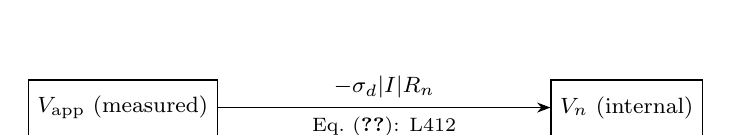
\begin{tikzpicture}[x=3.2cm,y=1.0cm,
  block/.style={rectangle,draw,minimum width=1.8cm,minimum height=0.7cm,
    align=center,font=\footnotesize}]
\node[block] (vapp) at (0,0) {$V_\app$ (measured)};
\node[block] (vn)   at (2,0) {$V_n$ (internal)};
\draw[-{Stealth}] (vapp) -- (vn)
  node[midway,above,font=\footnotesize]{$-\sigma_d|I|R_n$}
  node[midway,below,font=\scriptsize]{Eq.~\eqref{eq:vn}: L412};
\end{tikzpicture}
\caption{분극 변환 (N1). 인가 전위에서 IR 강하를 제거해 열역학 전위를 얻는다.
방전 시 $V_\app > V_n$, 충전 시 $V_\app < V_n$.}
\label{fig:polar}
\end{figure}

\begin{verifybox}
차원: $\sigma_d$[무차원]$\times|I|$[A]$\times R_n$[$\Omega$] $=$ V \checkmark.
극한: $|I|\to0$이면 $V_n\to V_\app$ (평형 OCV 회복).
부호: 방전에서 $V_n = V_\app - |I|R_n < V_\app$이므로 내부 전위가 측정 전위보다 낮다.
ICA peak는 $V_n = U_j^d$에서 발생하고, 이를 측정축으로 환원하면
$V_\app = V_n + |I|R_n > V_n$이므로, 방전 ICA peak는 OCV peak보다
\textbf{높은} 전위에 나타난다 \checkmark.
\end{verifybox}

% ====================================================================
\section{평형 중심 전위 $U_j(T)$ (N2)}
\label{sec:Uj}
% ====================================================================
앞 절에서 받은 것: $V_n$.
다음 절로 넘기는 것: 전이 $j$의 평형 중심 $U_j(T)$ (분기 중심 계산의 기반).

\subsection{열역학에서 $U_j(T)$까지}

삽입 반응 $\mathrm{Li}^++e^-+[\;]\rightleftharpoons\mathrm{Li}_{(\text{흑연})}$의
표준 Gibbs 자유에너지 변화는
\begin{equation}
  \Delta G_j = -\,F\,U_j,
  \label{eq:deltaG}
\end{equation}
로 전위 $U_j$와 연결된다.
Gibbs 항등식 $\Delta G = \Delta H - T\Delta S$를 적용하면:
\begin{equation}
  -F\,U_j = \Delta H_{\mathrm{rxn},j} - T\,\Delta S_{\mathrm{rxn},j},
\end{equation}
이를 $U_j$에 대해 정리하면
\begin{equation}
  \boxed{U_j(T) = \frac{-\Delta H_{\mathrm{rxn},j} + T\,\Delta S_{\mathrm{rxn},j}}{F}.}
  \label{eq:Uj}
\end{equation}
이것이 \texttt{func\_U\_j(T, dH\_rxn, dS\_rxn)} (L68)의 정확한 구현이다.
$\Delta H_{\mathrm{rxn},j} < 0$ (발열 삽입): 분자의 첫 항은 양수.
온도 의존성: $\partial U_j/\partial T = \Delta S_{\mathrm{rxn},j}/F$.

\subsection{온도 의존성과 코드 초기값}

$\Delta S_{\mathrm{rxn},j}$의 부호와 크기에 따라 $U_j(T)$가 온도와 함께
단조 증가(양의 엔트로피) 또는 감소(음의 엔트로피)한다.

\begin{center}
\renewcommand{\arraystretch}{1.3}
\begin{tabular}{cccccc}
\toprule
전이 & stage & $U$ (V) & $\Delta H_{\mathrm{rxn}}$ (J/mol) & $\Delta S_{\mathrm{rxn}}$ (J/mol/K)
  & $Q_j/Q_\cell$ \\
\midrule
1 & $4\!\to\!3$ & 0.210 & $-11700$ & $+29.0$ & 0.10 \\
2 & $3\!\to\!2\mathrm{L}$ & 0.140 & $-13500$ & $0.0$ & 0.12 \\
3 & $2\mathrm{L}\!\to\!2$ & 0.120 & $-13100$ & $-5.0$ & 0.25 \\
4 & $2\!\to\!1$ & 0.085 & $-13000$ & $-16.0$ & 0.50 \\
\bottomrule
\end{tabular}
\end{center}
출처: \texttt{GRAPHITE\_STAGING\_LIT} (L535--L564).
``U'' 열은 $T=298.15\,\mathrm{K}$에서 식~\eqref{eq:Uj}의 결과와 정합한다
(코드 L587: \texttt{func\_U\_j(298.15, dH\_rxn, dS\_rxn)} 검증).

\begin{verifybox}
전이 1 (T=298.15 K): $U_1 = (-(-11700)+298.15\times29.0)/96485
= (11700+8647)/96485 = 20347/96485 \approx 0.2109$ V
$\approx 0.210$ V (초기값과 정합) \checkmark.
전이 2 ($\Delta S=0$): $U_2 = 13500/96485 \approx 0.1399$ V $\approx 0.140$ V \checkmark.
\end{verifybox}

% ====================================================================
\section{히스테리시스 분기 (N3)}
\label{sec:hys}
% ====================================================================
앞 절에서 받은 것: $U_j(T)$.
다음 절로 넘기는 것: 방향별 분기 중심 $U_j^d$ (점유율 계산의 중심).

\subsection{정규용액 자유에너지와 상분리}

전이 $j$를 격자기체로 보면, 진행률 $\xi = 1-\theta$로 표현한
1몰당 자유에너지는
\begin{equation}
  \bar{g}_j(\xi) = g_j^0 + RT\big[\xi\ln\xi + (1-\xi)\ln(1-\xi)\big]
                 + \Omega_j\,\xi(1-\xi),
  \label{eq:gxi}
\end{equation}
이다. 상호작용 에너지 $\Omega_j > 0$이 크면 $\bar{g}_j$가 비단조(이중 우물)가 되어
상분리가 발생한다.

$\bar{g}_j''(\xi)=0$이 되는 두 변곡점(spinodal 점)은
\begin{equation}
  \xi_{s,j}^\pm = \frac12 \pm \frac12\,u_j, \qquad
  u_j \equiv \sqrt{1 - \frac{2RT}{\Omega_j}} \quad(\Omega_j > 2RT),
  \label{eq:spinodal}
\end{equation}
이며, $\Omega_j \le 2RT$이면 $u_j$가 허수라 spinodal 점이 없고 — 상분리 없음.

\subsection{spinodal 상한 gap의 닫힌 꼴}

비단조 등온선의 극대($\xi_{s,j}^-$)와 극소($\xi_{s,j}^+$)에서의 전위 차가
충방전 분기의 열역학 상한이다. 두 spinodal 점을 식~\eqref{eq:Uj}에서 유도한
평형 전위 표현에 대입하고 차를 취하면 [\texttt{func\_dU\_hys}, L123]:
\begin{equation}
  \boxed{\Delta U_j^\hys = \frac{2}{F}\Big[\Omega_j\,u_j - 2RT\,\mathrm{artanh}\,u_j\Big],
  \qquad u_j = \sqrt{1-\frac{2RT}{\Omega_j}}.}
  \label{eq:hysdU}
\end{equation}
$\Omega_j \le 2RT$이면 $\Delta U_j^\hys \equiv 0$ (명시 분기, 코드 L127).

\subsection{방향별 분기 중심}

실제 전극에서는 다입자 mosaic 효과와 핵생성 장벽 때문에
분기 폭이 spinodal 상한보다 좁다.
이를 축소 인자 $\gamma_j \in [0,1]$과 부분 cycle 인자 $h_\eta$로 표현하면
[\texttt{func\_U\_branch}, L133]:
\begin{equation}
  \boxed{U_j^d = U_j + \tfrac12\,\sigma_d\,h_\eta\,\gamma_j\,\Delta U_j^\hys.}
  \label{eq:hyscenter}
\end{equation}
방전($\sigma_d=+1$)에서 $U_j^d = U_j + \frac12\gamma_j\Delta U_j^\hys > U_j$,
충전($\sigma_d=-1$)에서 $U_j^d < U_j$ — 방전 peak가 더 높은 전위에 나타난다.
$\gamma_j=0$이면 분기 없음(단일 중심 $U_j$), $\gamma_j=1$이면 spinodal 상한.

코드에서 히스테리시스가 활성화되려면 \texttt{gamma != 0.0 and Omega > 0.0}
(L448--L454)이며, 이때 \texttt{hys\_shift = func\_U\_branch(T\_rep, 0.0, Omega, gamma, sigma\_d, h\_eta)}로 이동량을 계산한다.

\begin{figure}[h]
\centering
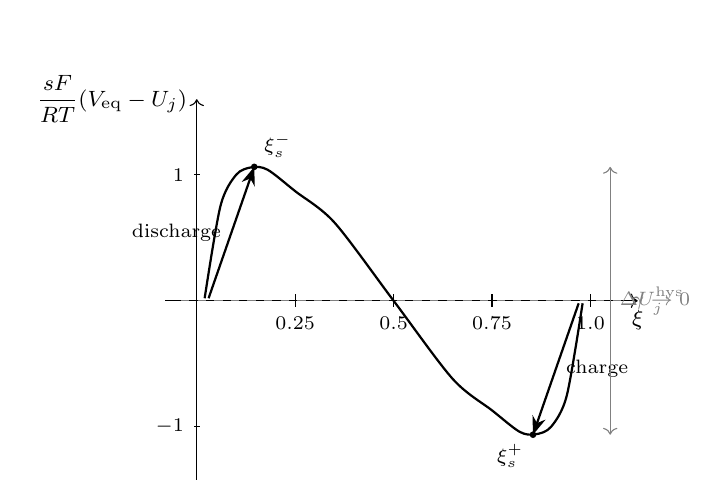
\begin{tikzpicture}[x=5.0cm,y=1.6cm]
\draw[->] (-0.08,0) -- (1.12,0) node[below] {\footnotesize $\xi$};
\draw[->] (0,-1.5) -- (0,1.6) node[left] {\footnotesize $\dfrac{sF}{RT}(V_{\eq}-U_j)$};
\foreach \xx in {0.25,0.5,0.75,1.0}
  {\draw (\xx,0.05) -- (\xx,-0.05) node[below] {\scriptsize $\xx$};}
\foreach \yy in {-1,1}
  {\draw (0.008,\yy) -- (-0.008,\yy) node[left] {\scriptsize $\yy$};}
% Omega=3RT equilibrium curve (approximate)
\draw[thick] plot[smooth] coordinates {
  (0.02,0.02)(0.06,0.75)(0.10,1.00)(0.14,1.06)(0.18,1.04)
  (0.25,0.87)(0.35,0.62)(0.50,0.0)
  (0.65,-0.62)(0.75,-0.87)(0.82,-1.04)(0.86,-1.06)(0.90,-1.00)(0.94,-0.75)(0.98,-0.02)};
% spinodal markers
\fill (0.146,1.063) circle (1.2pt) node[above right,font=\scriptsize]{$\xi_s^-$};
\fill (0.854,-1.063) circle (1.2pt) node[below left,font=\scriptsize]{$\xi_s^+$};
% arrows for discharge and charge overshoot
\draw[-{Stealth},thick] (0.03,0.02) -- (0.146,1.063)
  node[pos=0.5,left,font=\scriptsize]{discharge};
\draw[-{Stealth},thick] (0.97,-0.02) -- (0.854,-1.063)
  node[pos=0.5,right,font=\scriptsize]{charge};
% gap annotation
\draw[<->,gray] (1.05,-1.063) -- (1.05,1.063)
  node[pos=0.5,right,font=\scriptsize]{$\Delta U_j^\hys$};
% equilibrium axis
\draw[dashed,gray] (-0.04,0) -- (1.08,0) node[right,font=\scriptsize]{$\gamma\to 0$};
\end{tikzpicture}
\caption{비단조 평형 등온선 ($\Omega_j=3RT$, 개념도)과 과주행 경로.
방전은 spinodal $\xi_s^-$까지, 충전은 $\xi_s^+$까지 준안정 가지를 타므로
두 분기 중심이 $\Delta U_j^\hys$만큼 갈라진다.
실측 분기는 $\gamma_j$로 축소된다.}
\label{fig:vdwloop}
\end{figure}

\begin{verifybox}
$\Omega_j = 4RT_0$($T_0=298.15\,\mathrm{K}$)이면 $u=\sqrt{1-1/2}=0.707$,
$\mathrm{artanh}(0.707)\approx0.881$,
$\Delta U^\hys = (2/F)(4RT_0\times0.707 - 2RT_0\times0.881)
= (2RT_0/F)(4\times0.707 - 2\times0.881)
= (2RT_0/F)(2.828-1.762)
\approx 2.131\times(8.314\times298.15/96485)
\approx 54.9\,\mathrm{mV}$ \checkmark.
\end{verifybox}

% ====================================================================
\section{전이 폭과 평형 점유율 (N4, N5)}
\label{sec:width}
% ====================================================================
앞 절에서 받은 것: $U_j^d$ (분기 중심).
다음 절로 넘기는 것: $\xi_{\eq,j}(V_n)$ (평형 peak 및 꼬리 계산의 입력).

\subsection{폭 척도 $w_j$ — 통계역학 유도}

격자기체의 화학퍼텐셜은 $\mu_j(\xi) = \mu_j^0 + RT\ln[\xi/(1-\xi)] + \Omega_j(1-2\xi)$
이다. 평형 조건 $\mu_j = -F(V_n - U_j)$를 통해 정지점을 구하면,
이상 극한($\Omega_j=0$)에서 폭 척도는
\begin{equation}
  w_j = \frac{n_j RT}{F}
  \label{eq:wj}
\end{equation}
로 주어진다 [\texttt{func\_w}, L64]. 다중도 $n_j$는 전이 $j$의 격자 점유 구조를
반영하며 기본값은 $1$이다 [\texttt{\_n\_factor}, L274].

상호작용 에너지 $\Omega_j > 0$이 존재하면 중심 기울기 $\dd V_n/\dd\xi|_{\xi=1/2}$
가 깎여 유효 폭이 좁아진다. 이상 logistic 기울기 $4w_j$와 상호작용 수정 기울기
$(4RT-2\Omega_j)/F$를 등치하면:
\begin{equation}
  w_j^{\eff} = \frac{RT}{F}\!\left(1-\frac{\Omega_j}{2RT}\right)
  \label{eq:weff}
\end{equation}
[\texttt{func\_w\_eff}, L141]. $\Omega_j \to 2RT$에서 $w_j^{\eff}\to0$,
$\Omega_j > 2RT$이면 비단조(상분리 영역).
실제 코드에서 \texttt{use\_w\_eff=False}(기본값)이면 $w_j = n_j RT/F$,
\texttt{True}이면 $w_j^{\eff}$를 사용한다.

\subsection{logistic 평형 점유율}

정·역 속도 $r_j^\pm$의 균형(detailed balance)에서 정지점은, 전위-구동력
$\sigma_d F(V_n - U_j^d)$를 폭 $w_j$로 묶어 쓰면,
\begin{equation}
  \xi_{\sstat,j} = \frac{r_j^+}{r_j^+ + r_j^-}
  = \frac{\exp\!\bigl[\sigma_d(V_n-U_j^d)/w_j\bigr]}{1+\exp\!\bigl[\sigma_d(V_n-U_j^d)/w_j\bigr]}
  \label{eq:stationary}
\end{equation}
으로 유도된다. 정지점이 곧 평형 점유율이므로
\begin{equation}
  \boxed{\xi_{\eq,j}(V_n, T) = \frac{1}{1+\exp\!\big[-\sigma_d(V_n-U_j^d)/w_j\big]}.}
  \label{eq:xieq}
\end{equation}
이것이 \texttt{func\_ksi\_eq(T, V\_work, center, n\_j, sigma\_d)} (L84)의 구현이다.
방전($\sigma_d=+1$)에서 $V_n$ 증가 $\Rightarrow$ $\xi_{\eq,j}$ 증가
(탈리튬화 진행) \checkmark.

\begin{verifybox}
$V_n = U_j^d$에서 $\xi_{\eq,j} = \tfrac12$ (전이 중심).
$V_n \gg U_j^d$($\sigma_d=+1$)이면 $\xi_{\eq,j}\to1$; $V_n \ll U_j^d$이면 $\to0$.
$w_j = RT/F = 25.7\,\mathrm{mV}$ ($25^\circ\mathrm{C}$).
\end{verifybox}

% ====================================================================
\section{평형 peak (N6)}
\label{sec:eqpeak}
% ====================================================================
앞 절에서 받은 것: $\xi_{\eq,j}$, $w_j$.
다음 절로 넘기는 것: 평형 dQ/dV 기준선 (꼬리 없이 $|I|\to0$ 한계).

\subsection{$\xi_{\eq,j}$의 전압 미분 — 종 모양}

식~\eqref{eq:xieq}를 $z\equiv\sigma_d(V_n-U_j^d)/w_j$로 치환해 미분하면
\begin{equation}
  \frac{\dd\xi_{\eq,j}}{\dd z} = \xi_{\eq,j}(1-\xi_{\eq,j}),
\end{equation}
연쇄율 $\dd z/\dd V_n = \sigma_d/w_j$를 곱하면
\begin{equation}
  \frac{\dd\xi_{\eq,j}}{\dd V_n} = \frac{\sigma_d\,\xi_{\eq,j}(1-\xi_{\eq,j})}{w_j}.
  \label{eq:dxidV}
\end{equation}
$\xi(1-\xi)$는 $\xi=\tfrac12$에서 최대 $\tfrac14$인 종 모양이다.

\subsection{전하 보존과 ICA의 관계}

전하 보존식 $Q_\cell q = Q_\bg(V_n) + \sum_j Q_j\xi_j$를 미분하면
\begin{equation}
  \frac{\dd Q}{\dd V_n} = C_\bg + \sum_j Q_j\,\frac{\dd\xi_j}{\dd V_n}.
  \label{eq:dQdV}
\end{equation}
평형 추종($\xi_j = \xi_{\eq,j}$, $|I|\to0$) 극한에서 식~\eqref{eq:dxidV}를 대입하면
\begin{equation}
  \boxed{\frac{\dd Q}{\dd V_n}\bigg|_{\eq} = C_\bg + \sum_j Q_j\,
  \frac{\xi_{\eq,j}(1-\xi_{\eq,j})}{w_j}.}
  \label{eq:eqpeak}
\end{equation}
이것이 코드 \texttt{equilibrium()} (L354)과 \texttt{dqdv} L468의
\texttt{peak\_shape = ksi\_eq * (1 - ksi\_eq) / w}의 물리적 의미다.
peak 위치 $= U_j^d$, 높이 $= Q_j/(4w_j)$, 면적 $= Q_j$.
식~\eqref{eq:eqpeak}는 방향에 불변(평형은 방향 무관한 상태함수).

\begin{figure}[h]
\centering
\begin{tikzpicture}[x=0.7cm,y=16cm]
\draw[->] (-4.5,0) -- (5.5,0) node[below] {\footnotesize $(V_n-U_j^d)/w_j$};
\foreach \xx in {-4,-2,0,2,4}
  {\draw (\xx,0.006) -- (\xx,-0.006) node[below] {\scriptsize $\xx$};}
\draw[->] (-4.5,0) -- (-4.5,0.31) node[above] {\footnotesize $dQ/dV$ [arb.]};
% Logistic derivative bell: xi*(1-xi)/w -> 1/(4cosh^2(z/2)) shape
\draw[thick] plot[smooth] coordinates {
  (-4,0.0177)(-3,0.0452)(-2,0.105)(-1,0.1966)(0,0.25)
  (1,0.1966)(2,0.105)(3,0.0452)(4,0.0177)};
\node[font=\footnotesize] at (2.8,0.22) {$Q_j/(4w_j)$};
\draw[<->,gray] (-0.5,0.256) -- (0.5,0.256)
  node[pos=0.5,above,font=\scriptsize]{$\sim 4w_j$};
\draw[gray,dashed] (0,0) -- (0,0.26) node[above,font=\scriptsize]{$U_j^d$};
\node[font=\scriptsize] at (3.5,0.06) {area $=Q_j$};
\end{tikzpicture}
\caption{평형 peak (N6): $Q_j\xi_{\eq}(1-\xi_{\eq})/w_j$. 위치 $=U_j^d$,
높이 $=Q_j/(4w_j)$, 면적 $=Q_j$. 방향 불변(충방전 공통 기준선).}
\label{fig:eqpeak}
\end{figure}

% ====================================================================
\section{동역학 지연 길이 $L_V$ (N7)}
\label{sec:Lq}
% ====================================================================
앞 절에서 받은 것: $\xi_{\eq,j}$, $U_j^d$, $w_j$.
다음 절로 넘기는 것: $L_{q,j}$ 및 $L_{V,j}$ (인과 꼬리의 특성 길이).

\subsection{꼬리 컷점 affinity와 Butler--Volmer 속도}

전이 $j$의 꼬리는 $\xi_{\eq,j}$가 정점의 약 5\%로 떨어지는 컷점
($z = \sigma_d(V_n-U_j^d)/w_j = z_{\mathrm{cut}} = 4.357$, 기본값)에서 특성 길이를 결정한다.
이 컷점에서의 구동력(affinity)을 상한 $A_{\mathrm{cap}}$과 함께
\begin{equation}
  \mathcal{A} = \min\!\big(z_{\mathrm{cut}}\,n_j\,RT,\; A_{\mathrm{cap}}\,RT\big)
  \label{eq:affinity}
\end{equation}
로 정의한다 [\texttt{\_resolve\_lag\_length}, L335]. $\mathcal{A}$는 전이당 상수다 —
$V_n$이 아니라 피팅 파라미터 $z_{\mathrm{cut}}$·$A_{\mathrm{cap}}$·$n_j$·$T$만의 함수이므로
$L_{q,j}$ 계산에서 $V_n$ 의존성이 직접 들어가지 않는다.
물리적 동기로는 전위가 높을수록 컷점 구동력이 커지고 장벽이 낮아지는 경향이 있으나,
v11 코드에서는 이를 컷점 상수 $\mathcal{A}$로 고정 평가한다.

정·역 방향 속도 $r_j^\pm$의 Butler--Volmer 비대칭은
고개 위치 $\chi$(전달 계수)로 표현된다:
\begin{equation}
  r_j^+ \propto e^{-(\Delta G_{a,j}-\chi\mathcal{A})/RT},\qquad
  r_j^- \propto e^{-(\Delta G_{a,j}+(1-\chi)\mathcal{A})/RT}.
  \label{eq:bv}
\end{equation}
두 부호의 합이 $1$: $\chi + (1-\chi) = 1$ (detailed balance 강제).
여기서 $\mathcal{A}$는 식~\eqref{eq:affinity}의 컷점 상수다.

\subsection{방향별 전달 계수 $\chi_d$}

꼬리의 깊은 쪽에서 상호작용 에너지 $\Omega_j$가 장벽에 흡수된다.
방전 깊은 꼬리($\xi\to1$)는 $r^+$ 장벽, 충전 깊은 꼬리($\xi\to0$)는 $r^-$ 장벽이 율속이다:
\begin{equation}
  \chi_d = \begin{cases} \chi & \sigma_d \ge 0 \;\text{(방전)}\\ 1-\chi & \sigma_d < 0 \;\text{(충전)}\end{cases}
  \label{eq:chid}
\end{equation}
[\texttt{func\_chi\_d}, L155]. 이 $\chi_d$로 유효 활성화 엔탈피가
\begin{equation}
  \Delta H_{a,j}^{\eff} = \Delta H_{a,j} - \chi_d\,\Omega_j
  \label{eq:dHeff}
\end{equation}
[\texttt{func\_dH\_a\_eff}, L149]로 수정된다. 방전에서 $\chi_d=\chi$,
충전에서 $\chi_d=1-\chi$ — 두 방향에서 유효 장벽의 감소량이 대칭적으로 갈린다.

\subsection{용량축 꼬리 길이 $L_{q,j}$}

Eyring 속도식의 전이율 $k_0 = k_BT/h$와 식~\eqref{eq:bv}의 정방향 속도를 결합하면:
\begin{align}
  \ln L_{q,j} &= \ln\!\frac{T_*}{T} - \ln\!\big(1+e^{-\mathcal{A}/RT}\big)
    + \frac{\Delta H_{a,j}^{\eff}-\Delta S_{a,j}T}{RT} - \frac{\chi_d\mathcal{A}}{RT},
  \label{eq:lnLq}\\
  &\text{where}\quad T_* = \frac{|I|\,h}{Q_\cell\,k_B}.
  \notag
\end{align}
이를 지수화한 것이 \texttt{func\_L\_q(T, I, Q\_cell, dH\_a, dS\_a, x, A)} (L90)이다.
$L_{q,j} = |I|/(Q_\cell k_j)$ — 요구 전환율(전류)과 반응 공급(속도)의 비.
$\mathcal{A}$가 식~\eqref{eq:affinity}의 전위-무의존 상수이므로, $L_{q,j}$ 역시
$V_n$에 직접 의존하지 않는다(전위별 꼬리 길이 변화는 $\mathcal{A}$·$z_{\mathrm{cut}}$ 피팅으로 포착).

\subsection{전압축 꼬리 길이 $L_{V,j}$}

꼬리 컷점 $q_a$에서의 OCV 기울기 $|\dd V_n/\dd q|_{q_a}$[\texttt{dVdq\_qa}]로
용량축 길이를 전압축 길이로 환산한다 [L351]:
\begin{equation}
  L_{V,j} = \Big|\frac{\dd V_n}{\dd q}\Big|_{q_a} \cdot L_{q,j}.
  \label{eq:LV}
\end{equation}

\begin{verifybox}
차원: $L_{q,j} = [A\,\mathrm{s}]/([\mathrm{C}][\mathrm{s}^{-1}])$ = 무차원 \checkmark.
$L_{V,j}$ 차원: [V/무차원]$\times$무차원 = V \checkmark.
극한: $|I|\to0$이면 $T_*\to0$, $\ln L_{q,j}\to-\infty$,
$L_{q,j}\to0$ → 꼬리 없음 (평형 회복) \checkmark.
기호 일관성: 식~\eqref{eq:lnLq}의 $\mathcal{A}$는 식~\eqref{eq:affinity}의
컷점 상수로서 $V_n$ 무의존. 따라서 $\partial L_{q,j}/\partial V_n = 0$
(코드 L346: \texttt{func\_L\_q}는 $V_n$을 인자로 받지 않음) \checkmark.
충전 방향 ($\sigma_d=-1$): $\chi_d = 1-\chi$로 교체되어 $\Delta H_{a,j}^{\eff}$가
달라지고 $L_{q,j}$가 방전과 다른 값을 갖는다 \checkmark.
\end{verifybox}

% ====================================================================
\section{인과 기억 꼬리와 충전 격자 역전 (N8)}
\label{sec:tail}
% ====================================================================
앞 절에서 받은 것: $\xi_{\eq,j}$, $L_{q,j}$, $L_{V,j}$.
다음 절로 넘기는 것: \texttt{peak\_shape} = $(ξ_{\eq}-ξ_{\mathrm{lagged}})/L_V$ (peak 기여).

\subsection{일반 완화 방정식과 닫힌 해}

용량 좌표 $q$로 표현한 운동방정식은
\begin{equation}
  \frac{\dd\xi_j}{\dd q} = \frac{Q_\cell k_j}{|I|}\,(\xi_{\eq,j}-\xi_j)
  = \frac{1}{L_{q,j}}\,(\xi_{\eq,j}-\xi_j).
  \label{eq:relaxq}
\end{equation}
지연 $r_j = \xi_{\eq,j}-\xi_j$의 방정식이
\begin{equation}
  \frac{\dd r_j}{\dd q} = \frac{\dd\xi_{\eq,j}}{\dd q} - \frac{r_j}{L_{q,j}}
  \label{eq:Lq_eq}
\end{equation}
이다. 적분인자 $e^{q/L_{q,j}}$로 닫힌 해를 구하면
\begin{equation}
  r_j(q) = r_j(q_0)\,e^{-(q-q_0)/L_{q,j}}
  + \int_{q_0}^q e^{-(q-q')/L_{q,j}}\,\frac{\dd\xi_{\eq,j}}{\dd q'}\,\dd q'.
  \label{eq:memory}
\end{equation}
이 해는 (i) 초기 지연의 지수 감쇠와 (ii) 과거 평형 목표 변화율의 기억 합성곱으로 구성된다.

\subsection{지수 기억 필터 — 이산 구현}

연속 합성곱~\eqref{eq:memory}를 이산 전위 격자 위에서 구현하면
1차 IIR(무한 임펄스 응답) 저역통과 필터가 된다:
\begin{equation}
  \xi_{\mathrm{lagged},j}[k] = \alpha\,\xi_{\mathrm{lagged},j}[k-1]
  + (1-\alpha)\,\xi_{\eq,j}[k],\qquad
  \alpha = e^{-\Delta V/L_{V,j}},
  \label{eq:iir}
\end{equation}
여기서 $\Delta V$는 격자 간격이다.
이것이 \texttt{\_causal\_lowpass(source, grid\_step, lag\_length)} (L100)의 구현이다.

\subsection{충전 격자 역전 — ★핵심 부호 처리}

인과 필터~\eqref{eq:iir}는 ``진행 방향의 과거''를 기억해야 한다.
방전($\sigma_d=+1$)에서는 $V_n$ 증가 방향이 진행 방향이므로
격자가 오름차순 그대로다.
충전($\sigma_d=-1$)에서는 $V_n$ 감소 방향이 진행 방향이므로
격자를 뒤집어 필터 후 되돌린다 [L474--L477]:
\begin{equation}
  \xi_{\mathrm{lagged}} = \begin{cases}
    \texttt{\_causal\_lowpass}(\xi_{\eq},\;\Delta V,\;L_V) & \sigma_d \ge 0\\
    \texttt{\_causal\_lowpass}(\xi_{\eq}[::-1],\;\Delta V,\;L_V)[::-1] & \sigma_d < 0
  \end{cases}
  \label{eq:reverse}
\end{equation}
이 격자 역전이 없으면 충전에서 꼬리가 진행 반대 방향으로 생성되어
$\dd Q/\dd V < 0$인 비물리 결과가 나온다.
역전 후 충전 dQ/dV = 방전의 거울(양수 유지) \checkmark.

\subsection{peak 기여}

$L_{V,j}$가 최소 격자 간격 기준보다 작으면 (\texttt{min\_lag\_grid\_steps}) 꼬리 없이
평형 peak (N6)로 직접 복귀한다 [L466--L468]. 그 외에는:
\begin{equation}
  \text{peak\_shape}_j = \frac{\xi_{\eq,j} - \xi_{\mathrm{lagged},j}}{L_{V,j}}
  \label{eq:peakshape}
\end{equation}
[L479]. $L_{V,j}\to0$ 극한에서 $\xi_{\mathrm{lagged}} \to \xi_{\eq}$이므로
peak\_shape $\to 0/0$이나 L'H\^{o}pital로 식~\eqref{eq:dxidV}의 평형 peak가 회복된다.

\begin{figure}[h]
\centering
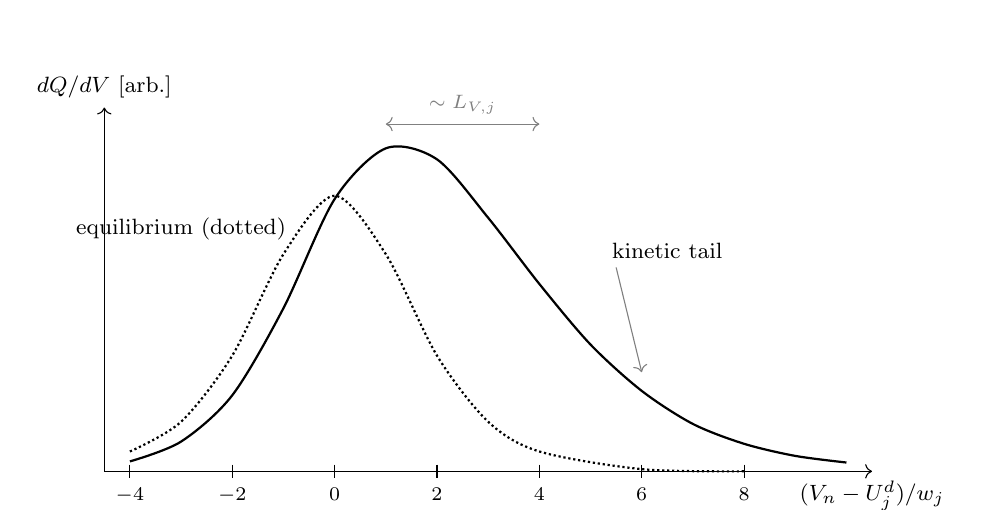
\begin{tikzpicture}[x=0.65cm,y=14cm]
\draw[->] (-4.5,0) -- (10.5,0) node[below] {\footnotesize $(V_n-U_j^d)/w_j$};
\foreach \xx in {-4,-2,0,2,4,6,8}
  {\draw (\xx,0.006) -- (\xx,-0.006) node[below] {\scriptsize $\xx$};}
\draw[->] (-4.5,0) -- (-4.5,0.33) node[above] {\footnotesize $dQ/dV$ [arb.]};
% equilibrium (reference, dotted)
\draw[densely dotted,thick] plot[smooth] coordinates {
  (-4,0.018)(-3,0.045)(-2,0.105)(-1,0.197)(0,0.25)
  (1,0.197)(2,0.105)(3,0.045)(4,0.018)(6,0.002)(8,0.0)};
% lagged (solid — shifted rightward, tail added)
\draw[thick] plot[smooth] coordinates {
  (-4,0.009)(-3,0.027)(-2,0.069)(-1,0.148)(0,0.247)(1,0.293)(2,0.283)
  (3,0.230)(4,0.170)(5,0.115)(6,0.073)(7,0.043)(8,0.025)(9,0.014)(10,0.008)};
% annotations
\node[font=\footnotesize] at (-3,0.22) {equilibrium (dotted)};
\node[font=\footnotesize] at (6.5,0.20) {kinetic tail};
\draw[->,gray] (5.5,0.185) -- (6.0,0.09);
\draw[<->,gray] (1,0.315) -- (4,0.315)
  node[pos=0.5,above,font=\scriptsize]{$\sim L_{V,j}$};
\end{tikzpicture}
\caption{인과 기억 꼬리 (N8). 점선: 평형 peak (N6 기준선).
실선: 지연된 곡선 --- peak가 진행 방향으로 이동하고
후방에 지수 꼬리가 형성된다. 꼬리 길이 $\sim L_{V,j}$.
방전 시 꼬리는 고전위 쪽(오른쪽), 충전 시 격자 역전 후 저전위 쪽.}
\label{fig:tail}
\end{figure}

\begin{verifybox}
충전 격자 역전 없이 $\sigma_d=-1$, $\xi_{\eq}$가 $V_n$ 감소 방향으로 증가하는 경우:
필터가 ``낮은 $V_n$의 과거''를 기억하여 $\xi_{\mathrm{lagged}} > \xi_{\eq}$가 될 수 있고
peak\_shape $< 0$ → $dQ/dV < 0$ (비물리).
역전 후: 진행 방향(낮은 $V_n$ 쪽)의 과거를 올바르게 기억 → peak\_shape $\ge 0$ \checkmark.
\end{verifybox}

% ====================================================================
\section{전이별 합산 — 최종 dQ/dV (N9)}
\label{sec:total}
% ====================================================================
앞 절에서 받은 것: 각 전이 $j$의 \texttt{peak\_shape}$_j$.
반환: $\dd Q/\dd V(V_\app)$.

\subsection{닫힌식 — 평형에서 지연을 뺀 것의 미분}

진행률 $\xi_j = \xi_{\eq,j} - r_j$ (지연 $r_j = \xi_{\eq,j}-\xi_j$)의 미분이
관측 ICA를 결정한다. 이를 전이별로 합산하면:
\begin{equation}
  \boxed{\frac{\dd Q}{\dd V_n} = C_\bg + \sum_{j=1}^{N_p} Q_j\,
  \frac{\xi_{\eq,j}-\xi_{\mathrm{lagged},j}}{L_{V,j}} = C_\bg + \sum_j Q_j\cdot\text{peak\_shape}_j.}
  \label{eq:closed}
\end{equation}
이것이 코드 \texttt{dqdv} L481의 \texttt{dqdv\_work += tr['Q'] * peak\_shape}
와 정확히 대응한다.

식~\eqref{eq:closed}는 두 극한에서 올바르게 환원된다:
\begin{itemize}[leftmargin=1.8em,itemsep=2pt]
\item $|I|\to0$: $L_{V,j}\to0$, $\xi_{\mathrm{lagged}}\to\xi_{\eq}$ 추종 → L'H\^{o}pital에 의해
  peak\_shape $\to \xi_{\eq}(1-\xi_{\eq})/w_j$ → 평형 peak 식~\eqref{eq:eqpeak}으로 환원.
\item $L_{V,j} < $ \texttt{min\_lag\_grid\_steps}$\times\Delta V$:
  코드 L466--L468에서 직접 $\xi_{\eq}(1-\xi_{\eq})/w$를 사용.
\end{itemize}

\subsection{전압축 역보간과 최종 반환}

작업 격자 $V_\mathrm{work}$ (패딩 포함)에서 계산한 \texttt{dqdv\_work}를
원래 측정 격자 $V_n$으로 역보간하고 [L483],
측정 전위 $V_\app = V_n + \sigma_d|I|R_n$으로 복귀한다:
\begin{equation}
  \frac{\dd Q}{\dd V_\app}\bigg|_{V_\app,i}
  = \mathrm{interp}\!\Big(V_{n,i},\;V_\mathrm{work},\;
    C_\bg + \sum_j Q_j\cdot\text{peak\_shape}_j\Big).
  \label{eq:interp}
\end{equation}

\subsection{staging 4전이 초기값표}

\texttt{GRAPHITE\_STAGING\_LIT} (L535--L564)에 담긴 흑연 4전이
초기값을 피팅 출발점으로 쓴다:

\begin{center}
\renewcommand{\arraystretch}{1.35}
\begin{tabular}{ccccccc}
\toprule
$j$ & stage & $U$ (V) & $\Omega$ (J/mol) & $\Delta H_a$ (J/mol) & $Q_j/Q_\cell$
  & \texttt{dVdq\_qa} (V) \\
\midrule
1 & $4\to3$ & 0.210 & 6000 & 48000 & 0.10 & 0.30 \\
2 & $3\to2\mathrm{L}$ & 0.140 & 8000 & 46000 & 0.12 & 0.30 \\
3 & $2\mathrm{L}\to2$ & 0.120 & 10000 & 44000 & 0.25 & 0.30 \\
4 & $2\to1$ & 0.085 & 13000 & 40000 & 0.50 & 0.30 \\
\bottomrule
\end{tabular}
\end{center}
$\Delta H_a$ 경향: stage 숫자 감소(만충 방향)로 장벽이 낮아진다 — DFT 계산과 정합.
이 값들은 초기값이며 Optuna 피팅으로 보정한다.

\subsection{세 인자 의존성 요약}

\begin{center}
\renewcommand{\arraystretch}{1.35}
\begin{tabular}{p{0.10\textwidth} p{0.28\textwidth} p{0.25\textwidth} p{0.25\textwidth}}
\toprule
& \textbf{온도 $T\downarrow$} & \textbf{C-rate $|I|\uparrow$} & \textbf{전위 $V\uparrow$}\\
\midrule
Peak 위치 & $U_j(T)$ 이동 (식~\eqref{eq:Uj}) & 분극 이동 (식~\eqref{eq:vn}) & 평형 중심 불변\\
꼬리 길이 & 지수 증가($e^{\Delta H_a/RT}$) & 비례 증가($\propto|I|$) & 직접 의존 없음($\mathcal{A}$ 고정)\\
Peak 높이 & 꼬리 경쟁으로 감소 & 감소 (지연 증가) & 꼬리 길이 불변, peak 이동만\\
\bottomrule
\end{tabular}
\end{center}

\begin{figure}[h]
\centering
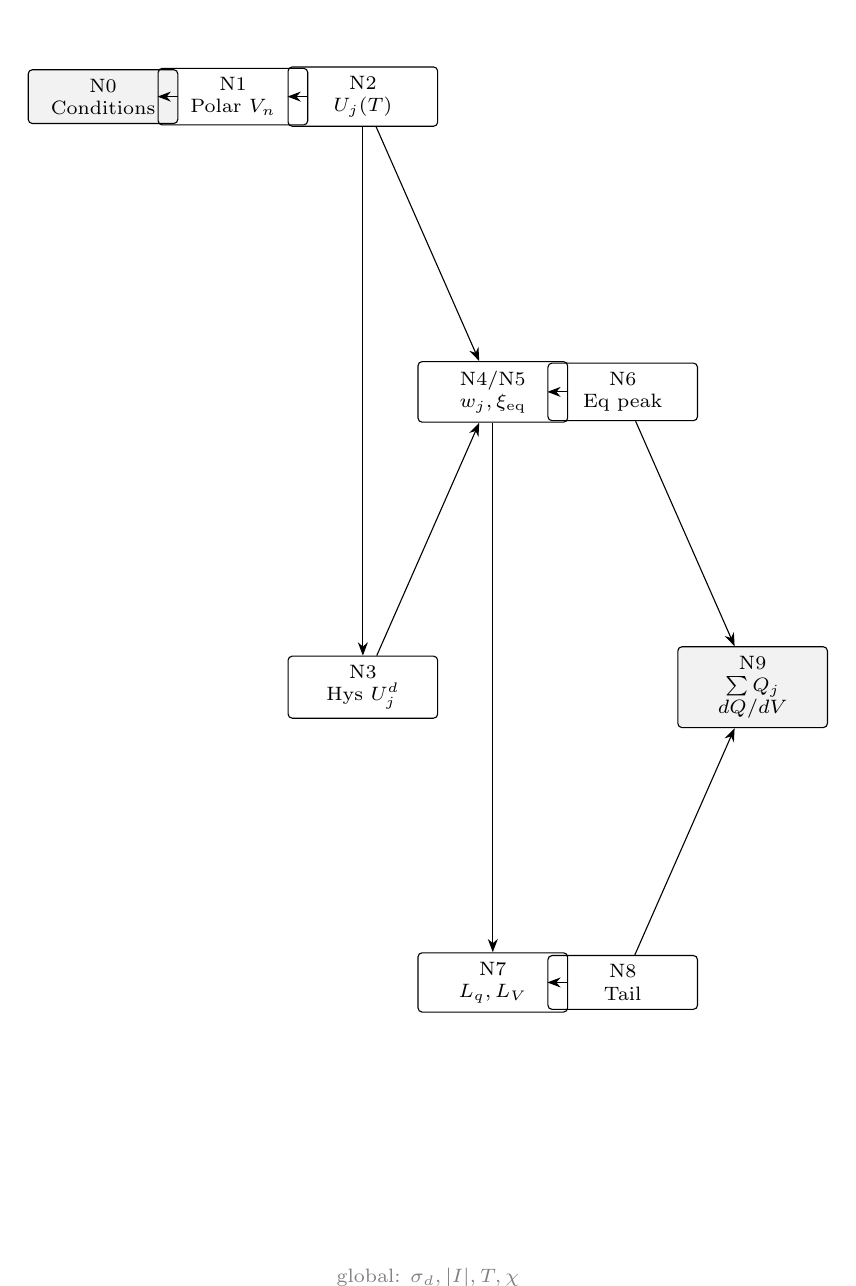
\begin{tikzpicture}[x=0.55cm,y=7.5cm,
  box/.style={draw,rectangle,rounded corners=1.5pt,minimum height=0.55cm,
    minimum width=1.9cm,align=center,font=\scriptsize}]
% Flow nodes
\node[box,fill=gray!10] (n0) at (0,0) {N0\\Conditions};
\node[box] (n1) at (3,0) {N1\\Polar $V_n$};
\node[box] (n2) at (6,0) {N2\\$U_j(T)$};
\node[box] (n3) at (6,-1) {N3\\Hys $U_j^d$};
\node[box] (n4) at (9,-0.5) {N4/N5\\$w_j,\xi_{\eq}$};
\node[box] (n6) at (12,-0.5) {N6\\Eq peak};
\node[box] (n7) at (9,-1.5) {N7\\$L_q,L_V$};
\node[box] (n8) at (12,-1.5) {N8\\Tail};
\node[box,fill=gray!10] (n9) at (15,-1) {N9\\$\sum Q_j$\\$dQ/dV$};
\draw[-{Stealth}] (n0) -- (n1);
\draw[-{Stealth}] (n1) -- (n2);
\draw[-{Stealth}] (n2) -- (n3);
\draw[-{Stealth}] (n3) -- (n4);
\draw[-{Stealth}] (n2) -- (n4);
\draw[-{Stealth}] (n4) -- (n6);
\draw[-{Stealth}] (n4) -- (n7);
\draw[-{Stealth}] (n6) -- (n9);
\draw[-{Stealth}] (n7) -- (n8);
\draw[-{Stealth}] (n8) -- (n9);
\node[font=\scriptsize,gray] at (7.5,-2.0) {global: $\sigma_d,|I|,T,\chi$};
\end{tikzpicture}
\caption{v11 코드 계산 진행 흐름 (N0$\to$N9). 각 노드는 본 문건의 절과 1:1 대응한다.
N3(히스테리시스)은 N2 출력을 받아 분기 중심 $U_j^d$를 수정하고,
N7은 N4/N5와 독립적으로 꼬리 길이를 계산한다.}
\label{fig:flowchart}
\end{figure}

% ====================================================================
\section{피팅 실행 지침 — 이 문건만으로 코드 재현}
\label{sec:fitting}
% ====================================================================
v11 곡선을 재현하는 코드는 다음 순서로 작성한다.

\textbf{모델 클래스 초기화.}
\texttt{GraphiteAnodeDischargeDQDV}(또는 동등 클래스)를
\texttt{GRAPHITE\_STAGING\_LIT} 초기값으로 생성한다.
반드시 지정해야 할 인자: \texttt{x}($\chi$, 기본 0.5),
\texttt{Rn}(분극 저항 [Ω]),
\texttt{Cbg}(배경 dQ/dV 값 또는 콜러블).

\textbf{곡선 계산 호출.}
\begin{itemize}[leftmargin=1.8em,itemsep=1pt]
\item 방전: \texttt{model.curve(V, direction="discharge", c\_rate=C, Q\_cell=Qc, T=T)}
\item 충전: \texttt{model.curve(V, direction="charge", c\_rate=C, Q\_cell=Qc, T=T)}
\item 또는 직접: \texttt{model.dqdv(V, T, I\_abs, Q\_cell, s=sigma\_d)}
\end{itemize}

\textbf{Optuna 피팅 파라미터 범위 (전이별).}
각 전이 $j$에 대해 최소한 다음을 자유 파라미터로 설정한다:
$U_j$ (초기값 ±50 mV 범위),
$\Omega_j$ (0 ~ 20000 J/mol),
$\Delta H_{a,j}$ (10000 ~ 80000 J/mol),
$\texttt{dVdq\_qa}$ (0.05 ~ 1.0 V).
전역 파라미터: $R_n$ (0 ~ 1 Ω), $\chi$ (0.3 ~ 0.7), $C_\bg$ (0 ~ 1).

\textbf{히스테리시스 활성화.}
충방전 gap이 측정될 때만 $\gamma_j > 0$, $\Omega_j > 2RT$ (~5000 J/mol 이상)으로 설정.
$\gamma_j=0$ (기본)이면 단일 중심.

\textbf{round-trip 검증.}
알려진 $\boldsymbol{\theta}^*$로 합성 곡선 생성 후 전 파이프라인이 $\boldsymbol{\theta}^*$를
회복하는지 확인(특히 충전 격자 역전 처리, 면적 보존 $\sum_j Q_j$).

% ====================================================================
\begin{thebibliography}{9}
\bibitem{dahn1991}
J.~R.~Dahn, ``Phase diagram of $\mathrm{Li}_x\mathrm{C}_6$,''
\emph{Phys.\ Rev.\ B} \textbf{44}, 9170 (1991).
DOI: 10.1103/PhysRevB.44.9170.

\bibitem{ohzuku1993}
T.~Ohzuku, Y.~Iwakoshi, K.~Sawai,
``Formation of Lithium--Graphite Intercalation Compounds in Nonaqueous Electrolytes,''
\emph{J.\ Electrochem.\ Soc.} \textbf{140}, 2490 (1993).
DOI: 10.1149/1.2220849.

\bibitem{eyring1935}
H.~Eyring, ``The Activated Complex in Chemical Reactions,''
\emph{J.\ Chem.\ Phys.} \textbf{3}, 107 (1935).
DOI: 10.1063/1.1749604.

\bibitem{bazant2013}
M.~Z.~Bazant,
``Theory of Chemical Kinetics and Charge Transfer based on Nonequilibrium Thermodynamics,''
\emph{Acc.\ Chem.\ Res.} \textbf{46}, 1144 (2013).
DOI: 10.1021/ar300145c.

\bibitem{dreyer2010}
W.~Dreyer \emph{et al.},
``The thermodynamic origin of hysteresis in insertion batteries,''
\emph{Nature Materials} \textbf{9}, 448 (2010).
DOI: 10.1038/nmat2730.

\bibitem{bloom2005}
I.~Bloom \emph{et al.},
``Differential voltage analyses of high-power, lithium-ion cells. 1,''
\emph{J.\ Power Sources} \textbf{139}, 295 (2005).
DOI: 10.1016/j.jpowsour.2004.07.056.

\bibitem{reynier2004}
Y.~Reynier, R.~Yazami, B.~Fultz,
``Thermodynamics of Lithium Intercalation into Graphites and Disordered Carbons,''
\emph{J.\ Electrochem.\ Soc.} \textbf{151}, A422 (2004).
DOI: 10.1149/1.1646152.
\end{thebibliography}

\end{document}
